\documentclass[14pt]{article}
\usepackage[colorlinks,allcolors=blue]{hyperref}
\usepackage{pdfpages}
\usepackage{graphics}
\usepackage{epsfig}
\usepackage{times}
\usepackage{amsmath}
\usepackage{subcaption}
\usepackage{multirow}
\usepackage{gensymb}
\usepackage{array}
\usepackage{float}
\usepackage{indentfirst}
\newcolumntype{P}[1]{>{\centering\arraybackslash}p{#1}}
\usepackage{booktabs, makecell}
\usepackage{diagbox}
\usepackage{float}
\floatstyle{plaintop}
\restylefloat{table}


\topmargin      0.0in
\headheight     0.0in
\headsep        0.0in
\oddsidemargin  0.0in
\evensidemargin 0.0in
\textheight     9.0in
\textwidth      6.5in

\title{{\bf CENG424 Embedded Computer Systems\\Final Exam Project Proposal \\ Spring 2022} \\ Group 9 \\
	\it Project Title: Soil Humidity Meter}


\date{\today}

\begin{document}

\pagestyle{plain}
\pagenumbering{roman}
\maketitle


\begin{figure}[H]
	\centering
	
\includegraphics[ scale = 0.35]{iyte_logo} 
\end{figure}

\textbf{ Group Members}
\begin{itemize}
	\item Student\_1 Arif Burak Demiray \& 250201022
	\item Student\_2 Ramazan Arslan \& 250201023 
	\item Student\_3 Burak Tutumlu \& 250201039
	\item Student\_4 Bekir Yörük \& 250201046
	\item Student\_5 Onur Cihangir \& 250201049
\end{itemize}



\cleardoublepage
\pagenumbering{arabic}

\abstract
In this project, we aim to measure the humidity levels around İzmir and how this humidity level is affected by the factors contributing to soil fertility and to inform how this productivity is kept at an optimum level. This project aims to improve over the years and increase humidity data more accurately. With this project, we are going to observe how the amount of humidity affects soils. We are going to be able to observe the humidity-soil fertility relationship and transfer the humidity content by analyzing the data in the system where we measure the humidity content of the soils in various regions with the tool we made with this project with Arduino.
\cleardoublepage

\section{Introduction}
In this project, we aim to measure the humidity information of the soil with the humidity meter sensor. By transferring this data to a cloud-based system, we aim to determine the difference in humidity between locations and to prepare a data on the factors affecting humidity. In this way, people who are interested in plant and garden works are going to be able to grow their soils in a healthier way, and those who want to access more detailed information about the relationship between soil and humidity are going to be able to develop more accurate products by using our data.

\section{Problem Definition}
One of the biggest problems that people experience while dealing with agriculture and plant breeding is that the factors that contribute to soil fertility cannot be kept at an optimum level. One of the most important of these factors is the humidity level. To measure this humidity level, people used various methods before. To give some examples, Gravimetric method, Electrical Resistance Method etc. But these are methods that are primitive in various aspects such as time or efficiency. This project of ours aims to provide users with information about their soil efficiently even without their plants, with a simple and easy-to-use device. In this context, we are going to transfer the information we have obtained with Arduino and soil humidity meter to the cloud system and provide access to it from mobile or web platform. With this solution, users are going to be able to access accurate humidity information about their plants in an instant and simple way. In addition, thanks to our project, people are going to be able to instantly compare their fields and plants in different locations, and thus our project is going to be a means of growing the plants in accordance with the conditions of the location.



\section{Stages}

\title{Sequence Diagram} 

\begin{figure}[H]
	\centering
	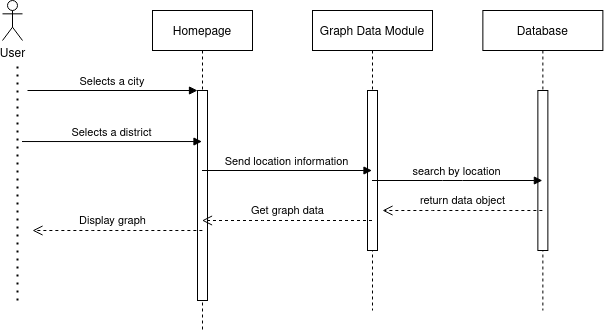
\includegraphics[ scale = 0.6]{seqdiagram.png} \newline\newline\newline\newline\newline\newline\newline\newline\newline\newline
\end{figure}


    \title{Flow Chart}

\begin{figure}[H]
	\centering
	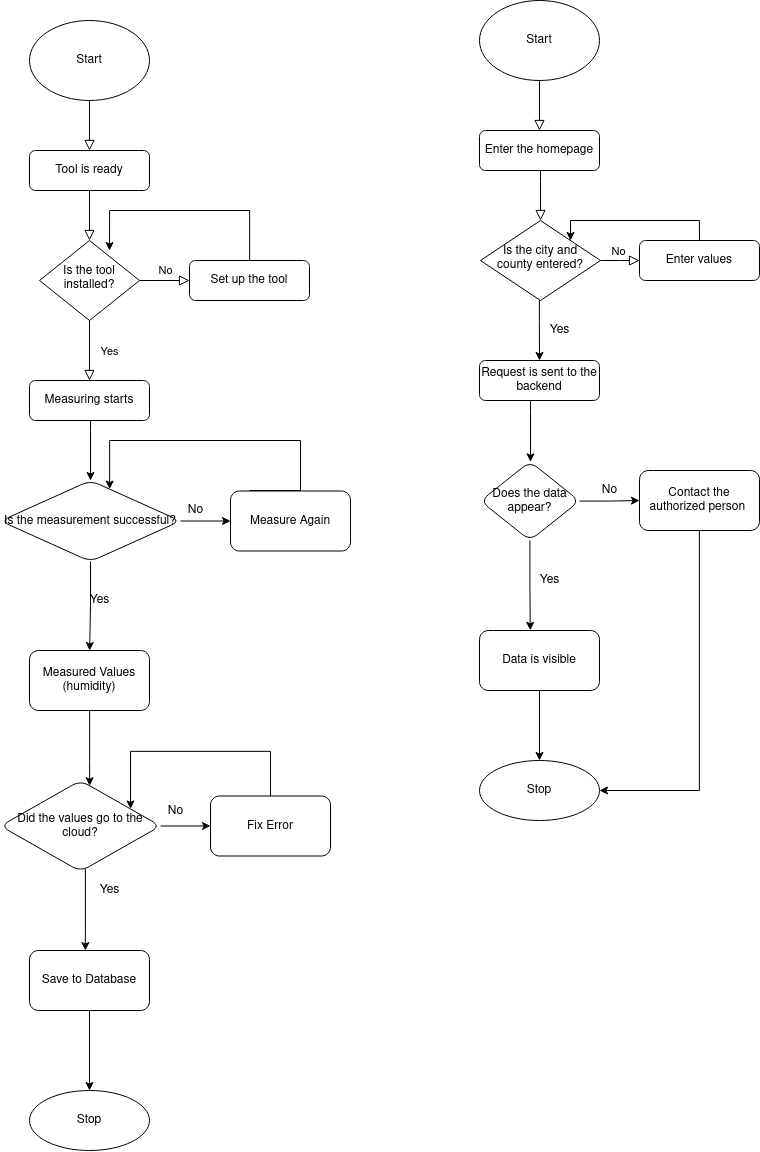
\includegraphics[ scale = 0.5]{flowchart.png}\newline\newline\newline
\end{figure}

\title{Use Case 1} 

\begin{figure}[H]
	\centering
	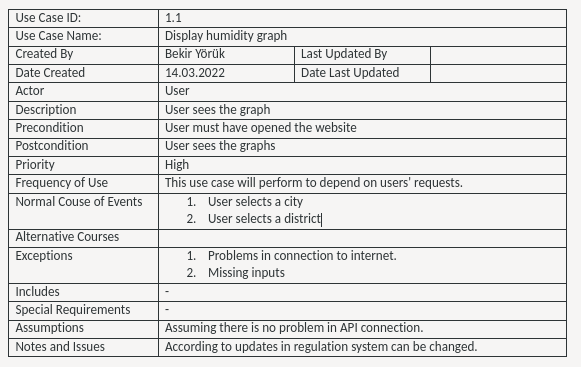
\includegraphics[ scale = 0.8]{usecase1.png} 
\end{figure}

\title{Use Case 2} 

\begin{figure}[H]
	\centering
	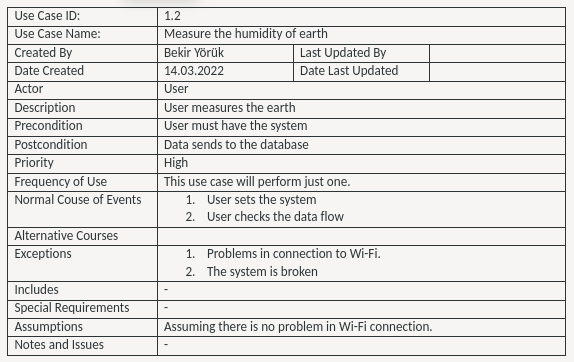
\includegraphics[ scale = 0.8]{usecase2.png} 
\end{figure}


\section{Tools, Software, Hardware}
We are going to use Jira for project management and GitHub for version control and code control. We are going to use React for the website. Backend is going to be nodejs or spring boot. Database is going to be MySQL because it is on free tier in AWS. Also, we are going to use AWS for the backend deployment and Vercel for the web deployment. We are going to use Ardunio for the soil humidity meter. It consist of lcd, buzzer, led lights, esp8266, ardunio uno, dht11 humidity sensor.

\begin{figure}[H]
	\centering
	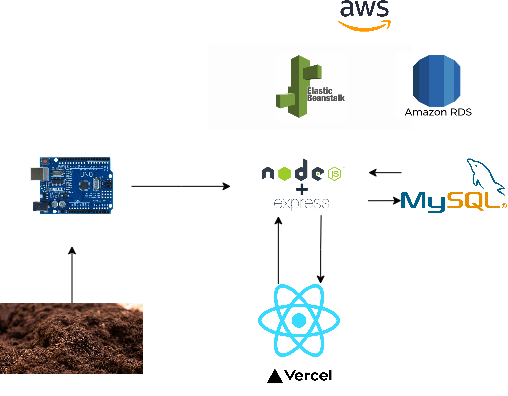
\includegraphics[ scale = 0.6]{sistemspecv2} 
\end{figure}


\section{Experiments\&Results, Test Phases}
Our garden is going to be the testing ground for this. We are going to use the device in three soil conditions: dry, wet and saturated with water. We plan to measure the humidity percentage and observe that the results go to our cloud server and access the results from the website. These test cases can be repeated morning, noon and evening. Response and request duration must be one second at maximum threshold. 
\section{Weekly Schedule}

\href{https://discord.gg/yA3v3fwm}{Discord} 
    
\href{https://eye-tracking-iyte.atlassian.net/jira/software/projects/SHM/boards/2}{Jira} 
    
\href{https://github.com/orgs/SoilHumidityMeter/dashboard}{GitHub} 
\\

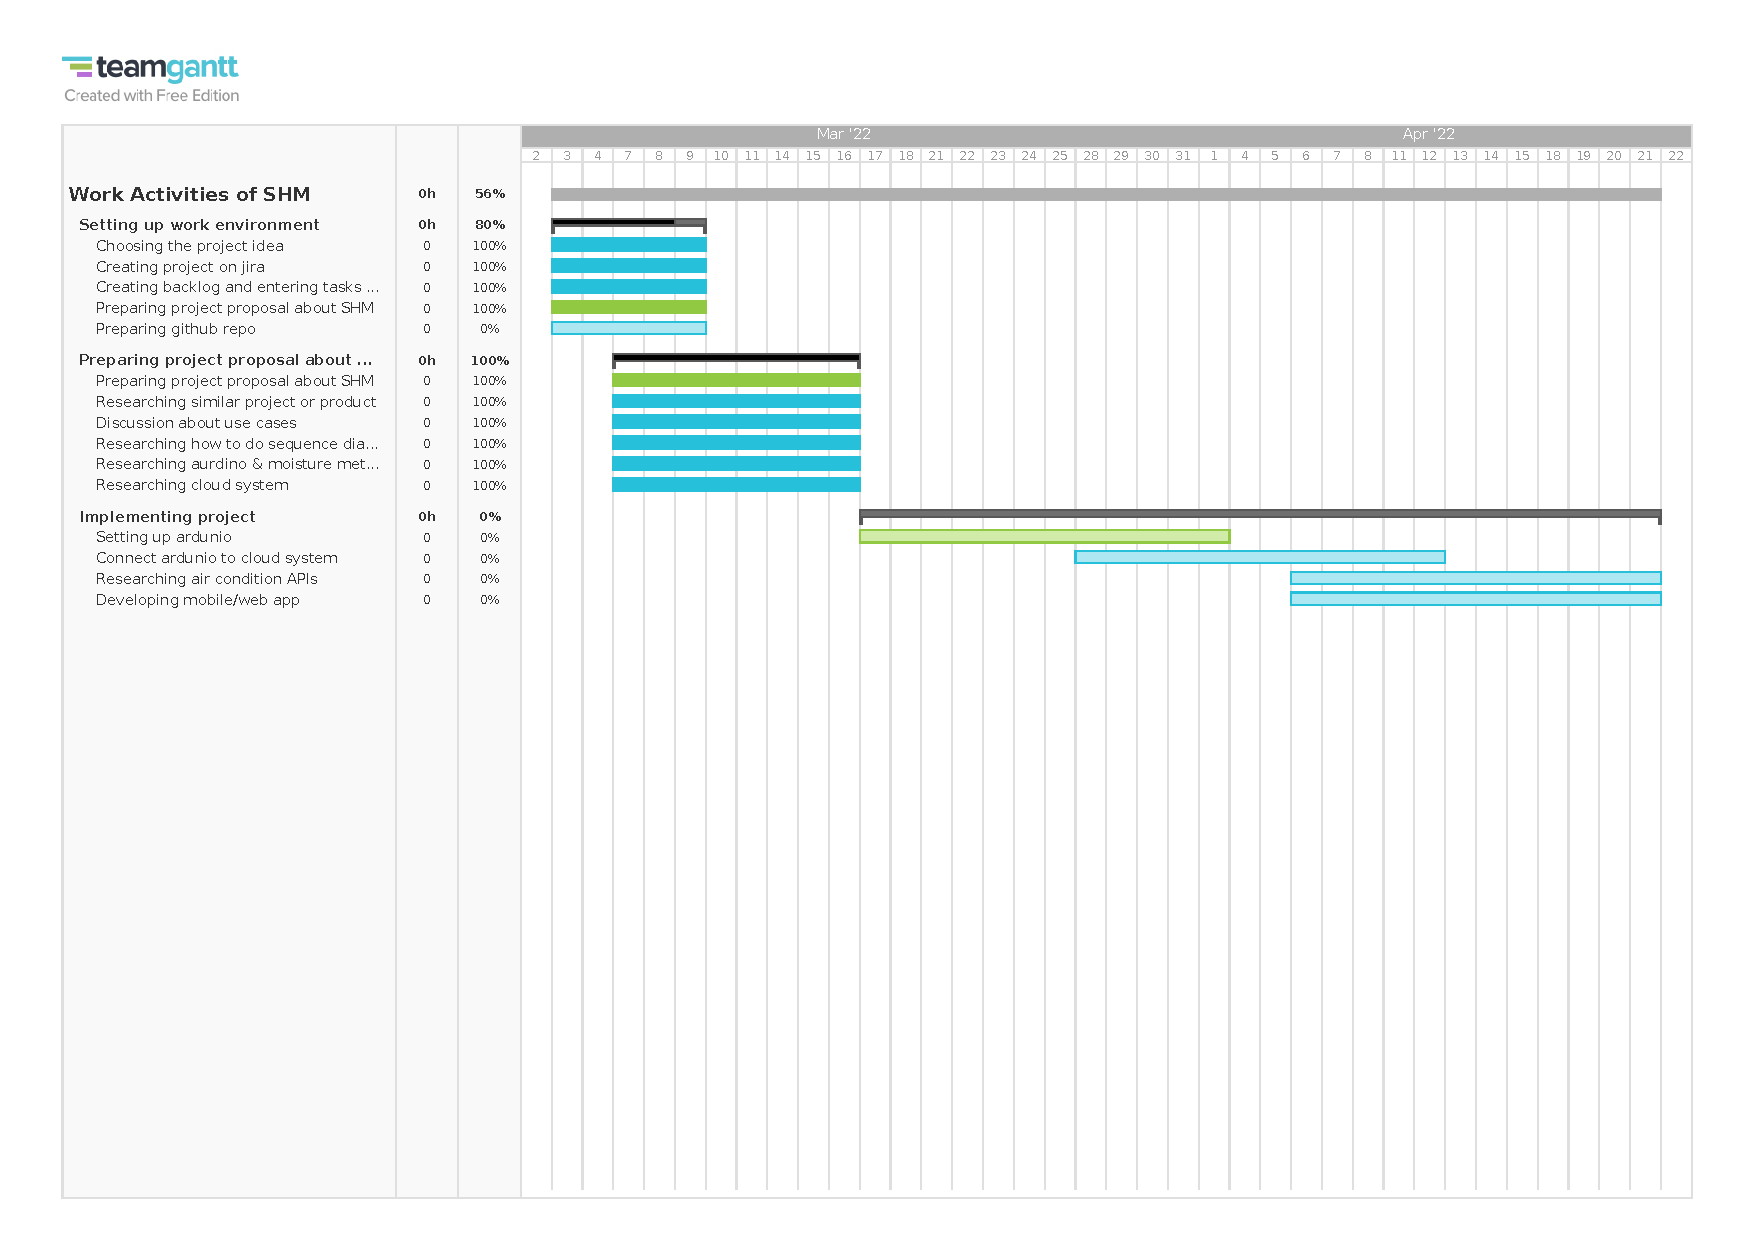
\includepdf[pages=-]{Work_Activities_of_SHM.pdf}


\end{document}


